\icode{N15L-EMI-MU-L2-261004-001}
\nceeID{2015山东}{unkown}
如图，一均匀金属圆盘绕通过其圆心且与盘面垂直的轴逆时针匀速转动，现施加一垂直穿过圆盘的有界匀强磁场，圆盘开始减速。在圆盘减速过程中，以下说法正确的是\paren[ABD]
	
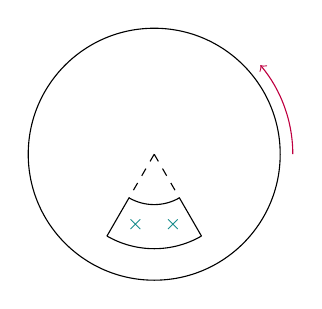
\begin{tikzpicture}[scale=.8,font=\scriptsize]
	\draw (0,0) circle(2);
	\draw (0,-.8) arc(-90:-60:.8);
	\draw (0,-.8) arc(-90:-120:.8);
	\draw (0,-1.5) arc(-90:-60:1.5);
	\draw (0,-1.5) arc(-90:-120:1.5);
	\draw (-120:.8)--(-120:1.5) (-60:.8)--(-60:1.5);
	\draw[dashed] (0,0)--(-120:.8) (0,0)--(-60:.8);
	\node at(-105:1.15)[teal]{\( \times \)};
	\node at(-75:1.15)[teal]{\( \times \)};
	\draw[->,purple] (2.2,0) arc(0:40:2.2);
\end{tikzpicture}
\begin{choices}
	\item 处于磁场中的圆盘部分，靠近圆心处电势高
	\item 所加磁场越强越易使圆盘停止转动
	\item 若所加磁场反向，圆盘将加速转动
	\item 若所加磁场穿过整个圆盘，圆盘将匀速转动
\end{choices}
\begin{answer}
    ABD\qquad 提示：
\end{answer}